\documentclass{article}
\usepackage{amsmath}
\usepackage{graphicx}
\usepackage{listings}
\usepackage{xcolor}
\usepackage{hyperref}
\usepackage[utf8]{inputenc}
\usepackage{float}
\usepackage{amsfonts}
\usepackage{amssymb}
\usepackage[a4paper, margin=1in]{geometry}

\lstdefinestyle{custom}{
    backgroundcolor=\color{lightgray!10},  % Couleur de fond légère
    basicstyle=\ttfamily\small,            % Police de base en taille petite
    breakatwhitespace=false,               % Ne pas couper les lignes aux espaces
    breaklines=true,                       % Couper les lignes longues
    captionpos=b,                          % Position de la légende
    commentstyle=\color{green!50!black},   % Style des commentaires
    keywordstyle=\color{blue},             % Style des mots-clés
    numberstyle=\tiny\color{gray},         % Style des numéros de ligne
    numbers=left,                          % Numéros de ligne à gauche
    showspaces=false,                      % Ne pas montrer les espaces
    showstringspaces=false,                % Ne pas montrer les espaces dans les chaînes
    showtabs=false,                        % Ne pas montrer les tabulations
    stringstyle=\color{red!50!brown},      % Style des chaînes de caractères
    tabsize=4                              % Taille des tabulations
}
\lstset{
  language=Python,
  basicstyle=\ttfamily\footnotesize,
  backgroundcolor=\color{gray!10},
  frame=single,
  keywordstyle=\color{blue},
  commentstyle=\color{green},
  stringstyle=\color{red},
  showstringspaces=false,
  style=custom
}

\begin{document}

\setlength\parindent{0mm}

\begin{titlepage}

    \begin{minipage}{0.3\linewidth}
     
\includegraphics[width=0.70\textwidth]{../images/logo_univ.png}   
    \end{minipage}
    \begin{minipage}{0.7\linewidth}
    \LARGE
            \textbf{Université de Montpellier} 
    \end{minipage}
    
    \begin{minipage}{0.3\linewidth}
     
\includegraphics[width=0.60\textwidth]{../images/logoSSD.png}   
    \end{minipage}
    \begin{minipage}{0.7\linewidth}
    \LARGE
            \textbf{Master 2 Statistiques et Sciences des Données}        
    \end{minipage}
    
    \vspace*{1cm}
    
        \begin{center}
         
            \Huge
    
    \hrulefill
            
            \textbf{TP : Support Vector Machine (SVM)}
    
    \hrulefill
                
                        
            \vspace{2cm}
    
            \Large
            \begin{minipage}[t]{0.4\textwidth}
                 \textbf{Auteur :}
            \end{minipage}
            \hfill
            \begin{minipage}[t]{0.45\textwidth}
                \raggedleft
                Maxence Lamure
            \end{minipage}
                
                
            \vspace{3cm}
            \large
            2024 - 2025
                
        \end{center}
    \end{titlepage}

\newpage
\renewcommand{\contentsname}{Table des matières}
\tableofcontents

\newpage

\section{Introduction aux SVM}
\hspace{7pt} Les Support Vector Machines (SVM) représentent une famille d'algorithmes d'apprentissage supervisé, largement utilisés pour les problèmes de classification et, dans une moindre mesure, de régression. Le principe des SVM repose sur la recherche d'un hyperplan séparateur optimal entre différentes classes de données. Cet hyperplan est défini de manière à maximiser la marge entre les points de chaque classe les plus proches de cette frontière, appelés vecteurs de support. La fonction de classification pour un SVM est donnée par :
\[
f(x) = \text{sign}\left(\sum_{i=1}^{n} \alpha_i y_i K(x_i, x) + b\right)
\]
où \(\alpha_i\) sont les coefficients du modèle, \(y_i\) les labels, \(K(x_i, x)\) est le noyau choisi, et \(b\) est le biais.\newline


\hspace{7pt} Dans le cas où les données sont linéairement séparables, le SVM détermine un hyperplan qui maximise la distance entre les vecteurs de support des différentes classes. Cependant, toutes les données ne sont pas toujours linéairement séparables. Pour répondre à cette problématique, les SVM utilisent la méthode du noyau (kernel) qui permet de transformer les données en un espace de dimension supérieure où une séparation linéaire devient possible.\newline

\hspace{7pt} Dans ce TP, nous allons principalement travailler avec deux types de noyaux :
\begin{itemize}
    \item Cas linéaire, adapté lorsque les données peuvent être séparées par un hyperplan.
    \item Cas polynomial, utile pour capturer des relations non linéaires en augmentant la complexité de la frontière.
\end{itemize}

\hspace{7pt} L'objectif de ce travail est de comparer les performances des SVM en fonction des noyaux utilisés et de l'ajustement de leurs hyperparamètres. En modifiant des paramètres comme le paramètre de régularisation ou les paramètres des noyaux, nous chercherons à comprendre comment ces manipulations influencent la qualité de la classification.

\section{Application}

\subsection{Question 1 : Noyau linéaire}
\hspace{7pt} À partir du code donnée en annexe, nous classifions la classe 1 contre la classe 2 en utilisant uniquement les deux premières variables caractéristiques de l'ensemble Iris et un noyau linéaire. Nous séparons équitablement les données d'entraînement et de test en deux échantillons distincts. Dans le cas d'un noyau linéaire, la fonction de noyau est définie comme suit :
\[
K(x, x') = \langle x, x' \rangle
\]
    
\hspace{7pt} L'analyse des résultats obtenus avec les paramètres suivants :
\begin{lstlisting}
parameters = {'kernel': ['linear'], 'C': list(np.logspace(-3, 3, 200))}
clf_linear = GridSearchCV(SVC(), parameters, cv=5)
clf_linear.fit(X_train, y_train)
\end{lstlisting}
montre que le modèle SVC avec noyau linéaire atteint un score de 72\% sur les données d'entraînement, mais ce score chute à 68\% sur les données de test, ce qui suggère un problème de généralisation. Cela pourrait indiquer un léger surentraînement ou une incapacité du modèle à capturer toute la complexité des données.

\subsection{Question 2 : Noyau polynomial}

\hspace{7pt} Nous utilisons un noyau polynomial pour comparer ses performances au noyau linéaire. Le noyau polynomial, permettant de capturer des relations non linéaires, est donné par :
\[
K(x, x') = (\alpha + \beta \langle x, x' \rangle)^\delta, \ \delta > 0
\]
    où \(\alpha\), \(\beta\), et \(\delta\) sont des paramètres ajustables.\newline

    \hspace{7pt}Le code suivant :
\begin{lstlisting}
parameters = {'kernel': ['poly'], 'C': Cs, 'gamma': gammas, 'degree': degrees}
clf_poly = GridSearchCV(SVC(), param_grid=parameters, n_jobs=-1)
clf_poly.fit(X_train, y_train)
\end{lstlisting}

permet de trouver les paramètres optimaux avec la validation croisée :

\begin{lstlisting}
{'C': 0.03162277660168379, 'degree': 1, 'gamma': 10.0, 'kernel': 'poly'\}
\end{lstlisting}

\hspace{7pt} Le modèle SVC avec un noyau polynomial atteint un score de 74\% sur les données d'entraînement et 72\% sur les données de test, ce qui montre une performance légèrement meilleure sur l'ensemble d'entraînement par rapport au modèle avec noyau linéaire, mais une performance de test comparable.\newline

\hspace{7pt} La Figure \ref{fig:noyaux} illustre les frontières de décision obtenues avec un noyau linéaire et un noyau polynomial, ainsi que la distribution des observations selon ces deux modèles.
    
\begin{figure}[H]
    \centering
    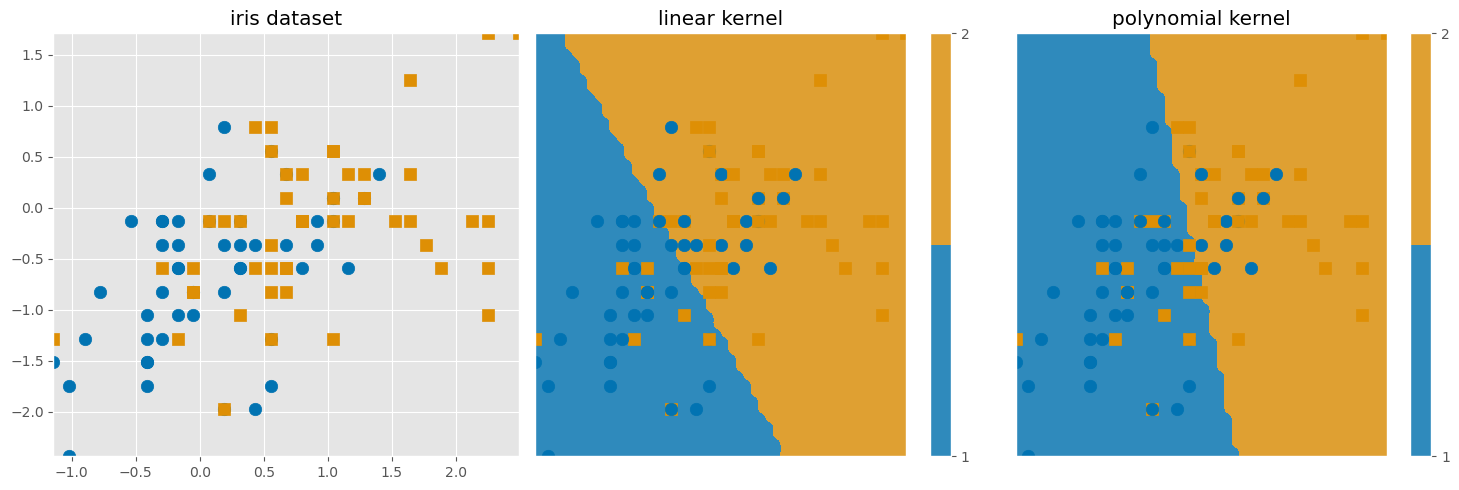
\includegraphics[width=1\textwidth]{../images/iris.png}
    \caption{\centering Performances des SVM appliqués au jeu de données iris pour un noyau linéaire et polynomial} 
    \label{fig:noyaux}
\end{figure}


\subsection{Question 3 : SVM GUI}

\hspace{7pt} En diminuant le paramètre $C$ dans un SVM avec un noyau linéaire, on observe que le modèle devient plus tolérant aux erreurs sur les données d'entraînement. Concrètement, cela se traduit par une marge plus large entre les classes, au prix de certaines mauvaises classifications. Le modèle privilégie ainsi une meilleure généralisation, en évitant de se concentrer trop strictement sur chaque point d'entraînement.  Ce compromis est représenté par le problème d'optimisation suivant :
\[
\min_{w, b, \xi} \frac{1}{2} \|w\|^2 + C \sum_{i=1}^{n} \xi_i
\]
sujet aux contraintes \(y_i (\langle w, x_i \rangle + b) \geq 1 - \xi_i\) et \(\xi_i \geq 0\).
\newline

\hspace{7pt} Dans le cadre d'un jeu de données déséquilibré, comme celui utilisé ici (90\% des points dans une classe et 10\% dans l'autre), une valeur plus faible de $C$ tend à favoriser la classe majoritaire. En effet, la frontière de décision devient moins précise et plus influencée par la majorité des points, ce qui peut entraîner une dégradation de la performance sur la classe minoritaire, avec davantage de points mal classifiés dans cette catégorie.

\section{Classification de visages}

\hspace{7pt} Pour classifier les visages, nous utilisons l'ensemble de données LFW (Labeled Faces in the Wild) puis nous sélectionnons deux personnes spécifiques (Tony Blair et Colin Powell) dont nous disposons au moins 70 photos et réduisons la taille des images par optimisation d'espace. Nous préparons ensuite les données dont un échantillon se trouve dans la Figure \ref{fig:lfw} pour une tâche de classification binaire.

\begin{figure}[H]
    \centering
    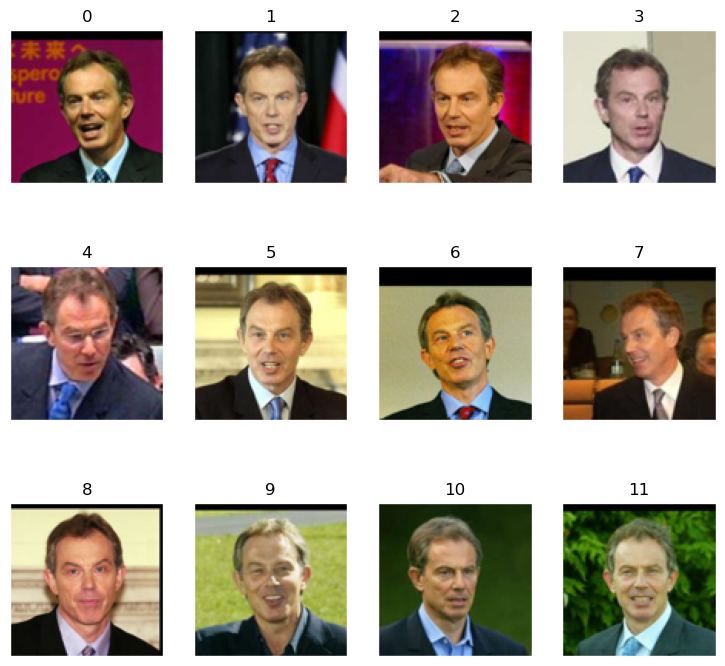
\includegraphics[width=0.6\textwidth]{../images/TB-CP.png}
    \caption{\centering Echantillon des données LFW} 
    \label{fig:lfw}
\end{figure}

\subsection{Question 4 : Paramètre de régularisation}

\hspace{7pt} Nous étudions l'influence du paramètre de régularisation C en ajustant les valeurs sur une échelle logarithmique entre $10^{-5}$ et $10^5$ et en observant les scores :

\begin{lstlisting}
Cs = 10. ** np.arange(-5, 6)
scores = []
for C in Cs:
    clf = SVC(kernel='linear', C=C)
    clf.fit(X_train, y_train)
    scores.append(clf.score(X_train, y_train)) 
\end{lstlisting}

\begin{figure}[H]
    \centering
    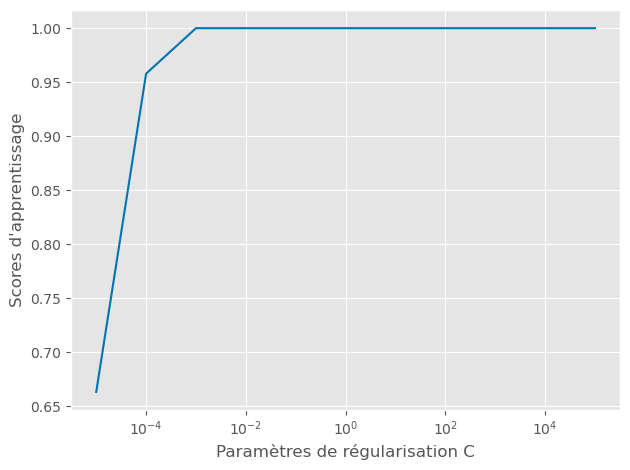
\includegraphics[width=0.7\textwidth]{../images/classification.png}
    \caption{\centering Graphe montrant le score d'apprentissage en fonction du paramètre de régularisation C} 
    \label{fig:score}
\end{figure}

\hspace{7pt} Comme montré dans la Figure \ref{fig:score}, le meilleur paramètre de régularisation est $C = 10^{-3}$, pour un score de 1. Ce score reste le même pour un C plus grand, ce qui montre la stabilité de la classification.\newline

\hspace{7pt} Nous réentraînons à présent le modèle avec ce C optimal et réalisons les prédictions finales sur les données de test. Nous comparons ensuite la précision obtenue à celle attendue d'un modèle prédictif aléatoire, servant de référence pour évaluer les performances.
\begin{lstlisting}
clf = SVC(kernel='linear', C=best_C)
clf.fit(X_train, y_train)
y_pred = clf.predict(X_test)

print("Chance level : %s" % max(np.mean(y), 1. - np.mean(y)))
print("Accuracy : %s" % clf.score(X_test, y_test))
\end{lstlisting}

\hspace{7pt} Nous obtenons alors une précision de 91\% et un niveau de chance de 62\%. Le modèle affiche donc une performance nettement meilleure que l'aléatoire, ce qui montre qu'il a bien appris à différencier les classes à partir des données fournies.\newline

\hspace{7pt} Les résultats sont illustrés dans la Figure \ref{fig:prediction} par le code suivant :

\begin{lstlisting}
prediction_titles = [title(y_pred[i], y_test[i], names)
                     for i in range(y_pred.shape[0])]

plot_gallery(images_test, prediction_titles)
\end{lstlisting}

\begin{figure}[H]
    \centering
    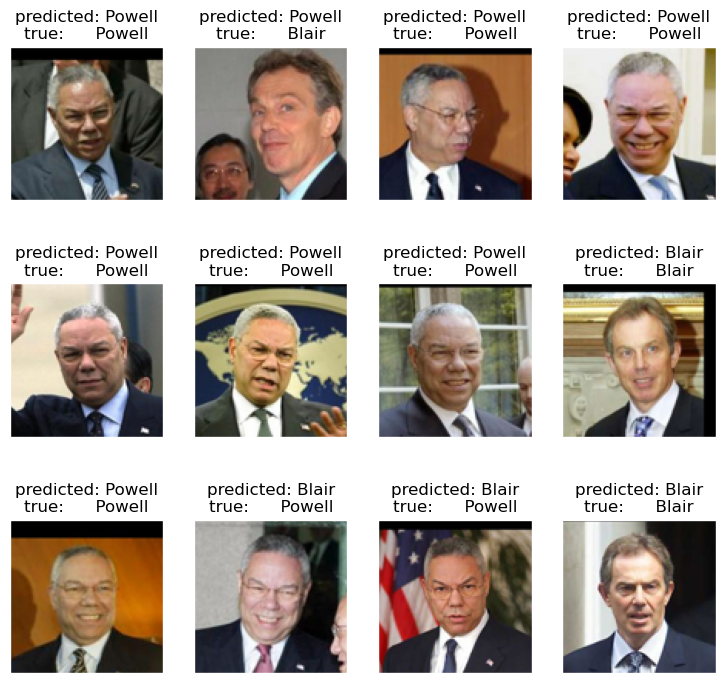
\includegraphics[width=0.6\textwidth]{../images/TB-CPpred.png}
    \caption{\centering Echantillon de prédiction du modèle pour les données LFW} 
    \label{fig:prediction}
\end{figure}

\hspace{7pt} La Figure \ref{fig:cc} présente quant à elle les coefficients du modèle linéaire appris sous forme de carte de chaleur sur une grille bidimensionnelle :

\begin{lstlisting}
plt.imshow(np.reshape(clf.coef_, (h, w)))
\end{lstlisting}

\begin{figure}[H]
    \centering
    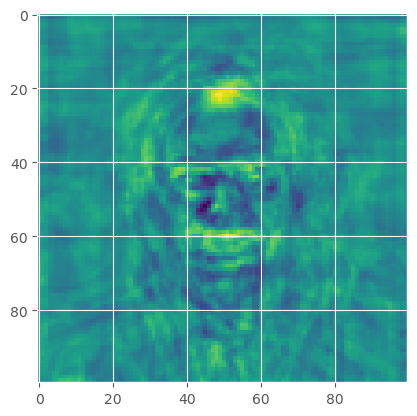
\includegraphics[width=0.5\textwidth]{../images/cc.png}
    \caption{\centering Coefficients du modèle linéaire appris sous forme de carte de chaleur} 
    \label{fig:cc}
\end{figure}

\hspace{7pt} Les variations de couleurs représentent les différences d'intensité des coefficients ou des données dans cette grille. Typiquement, des zones plus claires indiquent des valeurs plus élevées, tandis que des zones plus sombres signalent des valeurs plus faibles.\newline

\hspace{7pt} Nous constatons alors que le classifieur se base principalement sur certains éléments tels que l'implantation des cheveux au-dessus du crâne et sur les côtés, les sourcils/yeux, le nez et la bouche pour sa prédiction.

\subsection{Question 5 : Variables de nuisance}
\hspace{7pt} Nous ajoutons ici des variables de nuisance pour évaluer l'impact sur les performances du modèle dont le score est calculé par la fonction suivante :\newline
\begin{lstlisting}
def run_svm_cv(_X, _y):
    _indices = np.random.permutation(_X.shape[0])
    _train_idx, _test_idx = _indices[:_X.shape[0] // 2], _indices[_X.shape[0] // 2:]
    _X_train, _X_test = _X[_train_idx, :], _X[_test_idx, :]
    _y_train, _y_test = _y[_train_idx], _y[_test_idx]

    _parameters = {'kernel': ['linear'], 'C': list(np.logspace(-3, 3, 5))}
    _svr = svm.SVC()
    _clf_linear = GridSearchCV(_svr, _parameters)
    _clf_linear.fit(_X_train, _y_train)

    print('Generalization score for linear kernel: %s (train), %s (test) \n' %
          (_clf_linear.score(_X_train, _y_train), _clf_linear.score(_X_test, _y_test)))
\end{lstlisting}

\hspace{7pt} Sans variables de nuisance, le modèle atteint un score de 1 pour les données d'entraînement et de 93\% pour les données de test, montrant une très bonne performance et sa capacité à généraliser sur de nouvelles données.\newline

\hspace{7pt} Avec variables de nuisance en revanche, calculé selon :

\begin{lstlisting}
sigma = 1
noise = sigma * np.random.randn(n_samples, 300, )
X_noisy = np.concatenate((X, noise), axis=1)
X_noisy = X_noisy[np.random.permutation(X.shape[0])]
\end{lstlisting}

le modèle atteint certes un score de 1 pour les données d'entraînement mais chute significativement à 47\% pour les données de test (inférieur au niveau de chance à 62\%), indiquant une mauvaise robustesse face à de nouvelles données malgré une bonne performance pour les données d'entraînement.

\subsection{Question 6 : Réduction de dimensions ACP}
\hspace{7pt} Après avoir analysé l'impact des variables de nuisance sur les performances du modèle, il peut être utile d'étudier une autre technique de prétraitement des données : la réduction de dimensions. Grâce à l'Analyse en Composantes Principales (ACP), l'objectif est de diminuer le nombre de variables tout en conservant un maximum d'information. Cette approche peut améliorer la performance du modèle en éliminant le bruit et en simplifiant la structure des données. Nous appliquerons donc l'ACP sur les données bruitées pour évaluer son effet sur la précision du modèle SVM, en testant trois scénarios : 40, 80 et 120 composantes. Le code correspondant à l'application de l'ACP est le suivant :
\begin{lstlisting}
pca = PCA(n_components=n_components).fit(X_noisy)
X_pca = pca.transform(X_noisy)
\end{lstlisting}

\hspace{7pt} Ainsi, après un temps de calcul relativement long, on obtient les résultats suivants :
\begin{itemize}
    \item 40 composantes : 
    \begin{lstlisting}
    0.7473684210526316 (train), 0.5684210526315789 (test) 
    \end{lstlisting}
    \item 80 composantes :
    \begin{lstlisting}
    0.868421052631579 (train), 0.4789473684210526 (test) 
    \end{lstlisting}
    \item 120 composantes : 
    \begin{lstlisting}
    0.8631578947368421 (train), 0.5421052631578948 (test) 
    \end{lstlisting}
\end{itemize}

\hspace{7pt} On observe une tendance au sur-apprentissage à mesure que le nombre de composantes augmente. En effet, avec 80 et 120 composantes, le score d'entraînement reste élevé, mais le score de test diminue. Cela suggère que le modèle devient trop complexe et s'adapte trop étroitement aux données d'entraînement, au détriment de la généralisation sur des données non vues.
\newline

\hspace{7pt} La réduction du nombre de composantes à 40 permet d'obtenir un meilleur équilibre entre les scores d'entraînement et de test, bien que les scores globaux soient plus faibles que dans les cas avec plus de composantes. Cela montre que l'ACP aide à réduire le bruit et à améliorer la généralisation jusqu'à un certain point. Au-delà d'un certain nombre de composantes, l'ajout de plus de dimensions semble réintroduire du bruit ou rendre le modèle plus sujet au sur-apprentissage.

\end{document}
